%%%%%%%%%%%%%%%%%%%%%%%%%%%%%%%%%%%%%%%%%%%%%%%%%%%%%%%%%%%%%%%%%%%%%%%%%%%%%%%%
%% 实验报告模板.tex                                                           %%
%% author: hxp<hxp201406@gmail.com>                                           %%
%% 按照基础物理实验老师发的模板更改形成                                       %%
%%%%%%%%%%%%%%%%%%%%%%%%%%%%%%%%%%%%%%%%%%%%%%%%%%%%%%%%%%%%%%%%%%%%%%%%%%%%%%%%
%% 备注:刚刚的注释刚好是80行,编写代码的时候不要超过80行,就是你的代码不要超 %%
%% 过我注释里面最后面的“%”,超过请换行。                                      %%
%%%%%%%%%%%%%%%%%%%%%%%%%%%%%%%%%%%%%%%%%%%%%%%%%%%%%%%%%%%%%%%%%%%%%%%%%%%%%%%%
%% 模板现在开始,请根据注释把相应的位置更改成对应的内容                       %%
%%%%%%%%%%%%%%%%%%%%%%%%%%%%%%%%%%%%%%%%%%%%%%%%%%%%%%%%%%%%%%%%%%%%%%%%%%%%%%%%


\documentclass{ctexart}


\usepackage{ctex}
\usepackage{amsmath}
\usepackage{amsfonts}
\usepackage{amssymb}
\usepackage{wasysym}
\newcommand{\angstrom}{\text{\normalfont\AA}}  % 定义了原子物理的A
\usepackage{graphicx}
\usepackage{float}
\usepackage{geometry}
\geometry{a4paper,scale=0.8}  % 定义页面大小是A4,缩放是0.8
\usepackage{caption}
\usepackage{subcaption}
\usepackage{enumitem}

\newcommand*{\md}{\mathop{}\!\mathrm{d}}   % 定义微分算子,直立体的d
\newcommand*{\me}{\mathrm{e}}              % 定义自然对数e,同样应当是直立体

% 如果你想要每一段的开头不要空两格,注释掉下面这两行
% \usepackage{parskip}
% \setlength{\parindent}{0cm}

% 默认的\mathbf对希腊字母不生效,这里改下
\usepackage{bm}
\let\Oldmathbf\mathbf
\renewcommand{\mathbf}[1]{\boldsymbol{\Oldmathbf{#1}}}

% 表格默认格内内容和边框没有留出距离,显示分数的时候,分数的上下会贴到边框上
% 因此我增加了表格内容和边框的最短距离是5像素
\usepackage{cellspace}
\setlength{\cellspacetoplimit}{5pt}
\setlength{\cellspacebottomlimit}{5pt}

% \si命令是用来写单位的,单位需要和之前的数字有一个空格的距离,而且应当直立体
% 用法:5 \si{km/h}
\newcommand{\si}[1]{\  \mathrm{#1}}

% 日期不要显示
\date{}

\usepackage{fancyhdr}
\pagestyle{fancy}
\fancyhf{}
\lhead{本文档TeX源码地址:https://github.com/hxp-plus/Notes/tree/master/Physics-Experiment/实验报告}
\rfoot{第 \thepage 页}
\renewcommand{\headrulewidth}{1pt}
\renewcommand{\footrulewidth}{1pt}

%% 标题三号黑体,作者信息为班级姓名学号
\newcommand{\generatetitle}[6]{\title{\zihao{3}\heiti#1} \author{#2 \quad
    \quad #3 \quad\quad #4 \quad\quad #5 \quad\quad #6} \maketitle\thispagestyle{fancy}}

%% 所有的引言、实验内容与数据处理啥的,用section
\ctexset {
  section = {
    format = \raggedright\zihao{4}\heiti,  % 设置所有section的字号为四号黑体左对齐
    name={,、},                            % 序号后跟顿号
    aftername={\hspace{0pt}},              % 修改序号和标题直接的间距为零
    number=\chinese{section},              % 设置序号为中文
  },
  subsection = {
    format = \raggedright\zihao{5}\heiti,  % 设置所有subsection的字号为五号黑体左对齐
    number={},              % 设置序号为没有序号
  }
}

%% 实验背景、实验目的啥的,用subsection
\ctexset {
  subsection = {
    format = \raggedright\zihao{5}\heiti,  % 所有subsection的字号为五号黑体左对齐
    number={},                             % 设置序号为没有序号
  }
}

%% 把subsection之间加上中括号
\let\oldsubsection\subsection
\renewcommand{\subsection}[1]{\oldsubsection{\!\!\!\!\!\!【#1】}}

%% 摘要和关键词用paragraph

\ctexset {
  paragraph = {
    format = \raggedright\zihao{5}\heiti,  % 所有paragraph的字号为五号黑体左对齐
    number={},                             % 设置序号为没有序号
  }
}

%% 把paragraph之间加上中括号
\let\oldparagraph\paragraph
\renewcommand{\paragraph}[1]{\oldparagraph{#1:\!\!\!\!\!\!}}

%% 再把参考文献的序号去掉
\makeatletter
\renewcommand\@biblabel[1]{}
\makeatother

\begin{document}

\generatetitle{综合物理实验报告——
  数字全息及实时光学再现}{物理4+4}{胡喜平}{U201811966}{hxp201406@gmail.com}{https://hxp.plus/}

\paragraph{摘要}
对于传统的照片而言,照片仅仅能记录图像在每一点光强大小的信息,不能记录光的相位信息,因此照片找出来的图像没有立体感。全息图像利用光的干涉原理,将图像的相位信息转化成光强信息,并记录光强,从而实现了用摄像机记录光的相位和光强的全部信息。本次实验搭建光路,使用摄像机记录了全息图,并且实现了全息图到原图的转换。

% 关键词
\paragraph{关键词}
全息图、数字全息

\section{实验原理}

\subsection{全息图的记录}

由惠更斯-菲涅尔原理可知,任何物体发出的光波可以看成是由物体上各点发出的球面波总和。光的电场分布可以由复振幅表示为

\begin{equation}
  \vec{E}_o \left( \vec{r} \right) = A_o \left( \vec{r} \right)  \exp \left[ - i \varphi_o \left( r \right) \right]
\end{equation}
但是传统相机都只能记录光强不能记录相位,因此相片没有立体感。

要想记录光的全部信息,需要借助全息图。常用的方法是干涉法,使具有振幅和相位信息的物体发出的光,和一束参考光干涉,参考光的振幅相位已知,测量到的干涉光的相位振幅已知,因此能反推出物体发出的光的相位和振幅。

假设物光$\vec{E}_o$和参考光$\vec{E}_r$照射在一个感光材料上,感光材料可以记录光强,其中

\begin{equation}
  \label{eq:物光}
  \vec{E}_o \left( x, y \right) = A_o \left( x, y \right) \exp \left[ - i \varphi_o \left( x, y \right) \right]
\end{equation} 

\begin{equation}
  \label{eq:参考光}
  \vec{E}_r \left( x, y \right) = A_r \left( x, y \right) \exp \left[ - i \varphi_r \left( x, y \right) \right]
\end{equation}

这两束光叠加后产生的光强是

\begin{equation}
  I = \left( \vec{E}_o + \vec{E}_r \right) \left( \vec{E}_o + \vec{E}_r \right)^{*} = E_o^2 + E_r^2 + \vec{E}_o \vec{E}_r^{*} + \vec{E}_o^{*} \vec{E}_r
\end{equation}

代入\ref{eq:物光}和\ref{eq:参考光},得出

\begin{equation}
  \label{eq:全息图记录}
  I \left( x, y \right) = A_o^2 + A_r^2 + A_o A_r \left\{ \exp \left[ i \left( \varphi_r - \varphi_o \right) \right] + \exp \left[ i \left( \varphi_o - \varphi_r \right) \right] \right\}
\end{equation}

可以看出,参考光的引入,使得物光的相位信息被转化成了光强,因此可以被感光的芯片或者电子元器件捕获。

将记录介质曝光即可得到全息图,其中全息图上每一点的振幅透射系数和曝光时的光强成线性关系,
即

\begin{equation}
  \label{eq:线性关系}
  t \left( x,y \right) = \beta_0 + \beta I \left( x, y \right)
\end{equation}

\subsection{全息图的再现}

将感光介质生成的全息图放在透射式空间光调制器上,另照射到透射式空间光调制器的再现光为

\begin{equation}
  \label{eq:再现光}
  \vec{E}_r' \left( x,y \right) = A_r' \exp \left( - i \varphi_r' \right)
\end{equation}

则经过空间调制器后光的复振幅为

\begin{equation}
  \label{eq:投射复振幅}
  \vec{E}_g \left( x,y \right) = \vec{E}_r' t
\end{equation}

将\ref{eq:全息图记录}、\ref{eq:再现光}和\ref{eq:线性关系}代入,得到

\begin{equation}
  \label{eq:全息再现}
  \vec{E}_g = A_r' \exp \left( - i \varphi_r' \right) \left[ \beta_0 + \beta \left( A_o^2 + A_r^2 + A_o A_r \left\{ \exp \left[ i \left( \varphi_r - \varphi_o \right) \right] + \exp \left[ i \left( \varphi_o - \varphi_r \right) \right] \right\} \right) \right]
\end{equation}

当复现光和参考光相位相同,即$\varphi_r = \varphi_r'$时

\begin{equation}
  \label{eq:复现光参考光相等}
  \vec{E}_g \left( x,y \right) = \left( \beta_0 + \beta A_o^2 + \beta A_r^2 \right) \vec{E}_r'
  + \beta A_r A_r' \vec{E}_o + \beta A_r A_r' \vec{E}_o^{*} \exp \left[ - 2 i \varphi_r \right]
\end{equation}

第一项是投射过来的复现光,算噪声。第二项是沿着原来物光传播方向传播的投射光,呈原来物体的虚像。第三项是物光的共轭光波,在原来物体对称位置呈实像。

\section{实验内容}

\begin{itemize}
\item 计算机模拟全息(数字记录,数字再现)
\item 可视数字全息(数字记录,光学再现)
\item 数字全息(光学记录,数字再现)
\item 实时传统全息(光学记录,光学再现)
\end{itemize}

\section{实验结果的分析和结论}

\subsection{计算机模拟全息}

不借助光学器件,用计算机模拟生成全息图并且在之后根据模拟出来的全息图重建图像,先研究全息图大概是什么样子的,以及全息图重建后应当是什么样子的。

我们用计算机模拟得到了下面五组图像,从做到右分别是输入的原图、计算机模拟得到的全息图、计算机根据模拟得出的全息图重建的图像。

\begin{figure}[H]
  \centering
  \begin{subfigure}{.32\textwidth}
    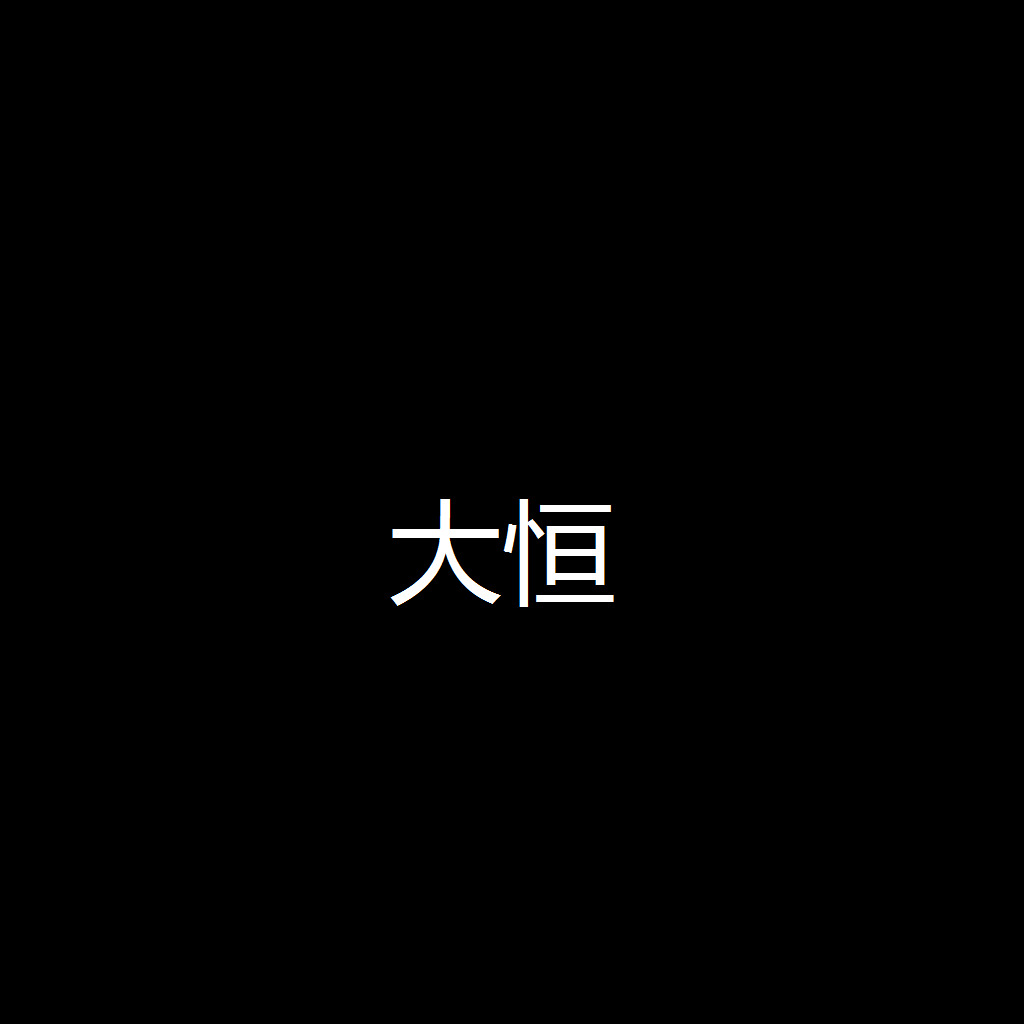
\includegraphics[width=\linewidth]{数字全息实验数据/计算机模拟全息/全息样品图片/1-大恒.jpg}
    \subcaption{使用的原图}
  \end{subfigure}
  \begin{subfigure}{.32\textwidth}
    
\includegraphics[width=\linewidth]{数字全息实验数据/计算机模拟全息/用软件模拟得到的全息图/1-大恒-全息图.jpg}
    \subcaption{计算机模拟的全息图}
  \end{subfigure}
  \begin{subfigure}{.32\textwidth}
    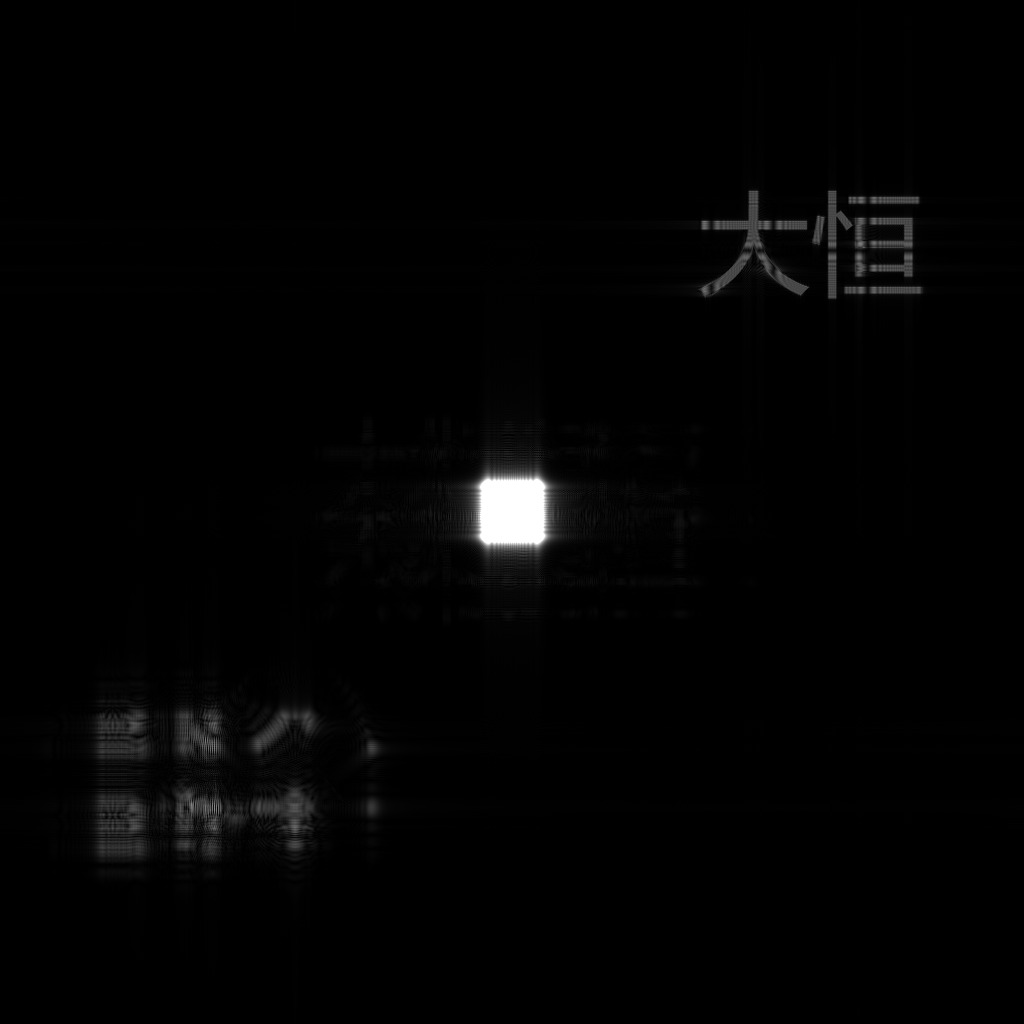
\includegraphics[width=\linewidth]{数字全息实验数据/计算机模拟全息/用软件重建的结果图像/1-大恒-重建.jpg}
    \subcaption{计算机重建结果}
  \end{subfigure}
  \caption{计算机模拟全息实验图像-大恒}
\end{figure}

\begin{figure}[H]
  \centering
  \begin{subfigure}{.32\textwidth}
    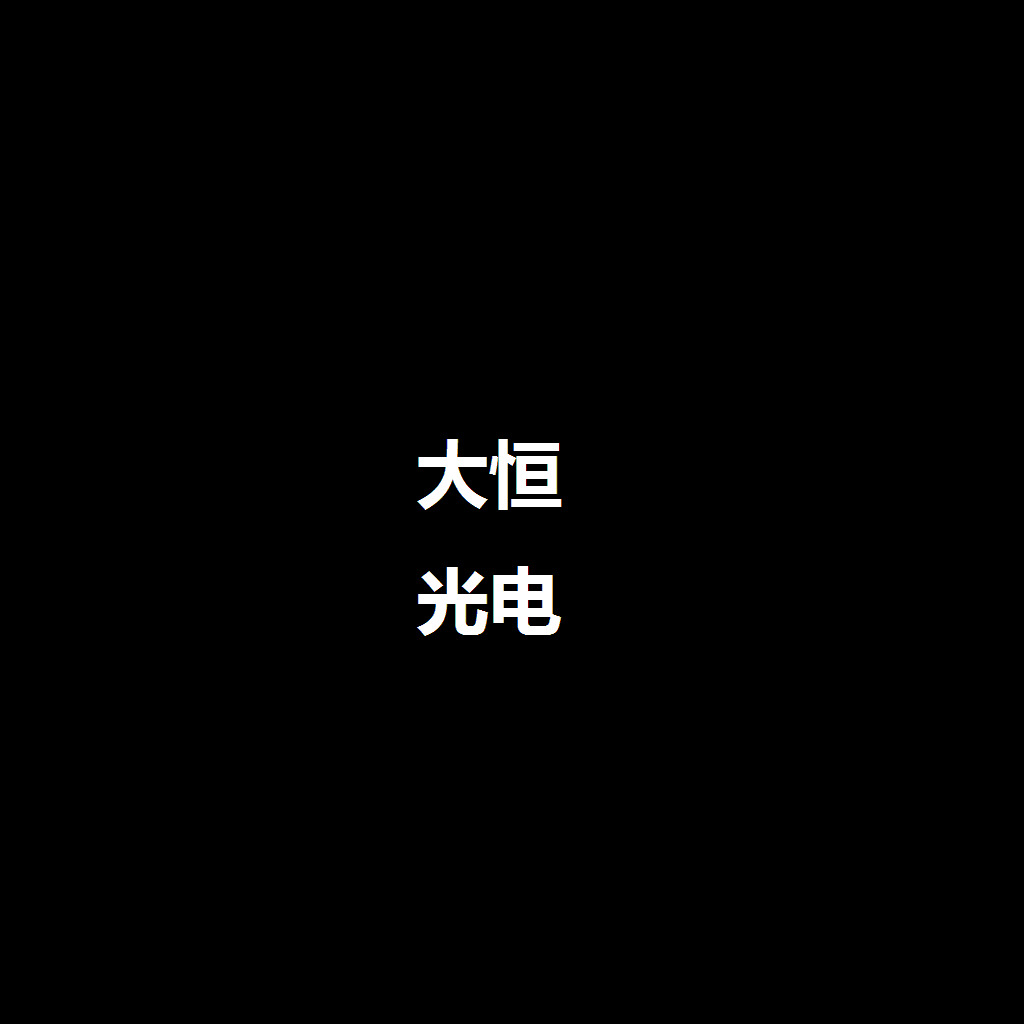
\includegraphics[width=\linewidth]{数字全息实验数据/计算机模拟全息/全息样品图片/2-大恒光电.jpg}
    \subcaption{使用的原图}
  \end{subfigure}
  \begin{subfigure}{.32\textwidth}
    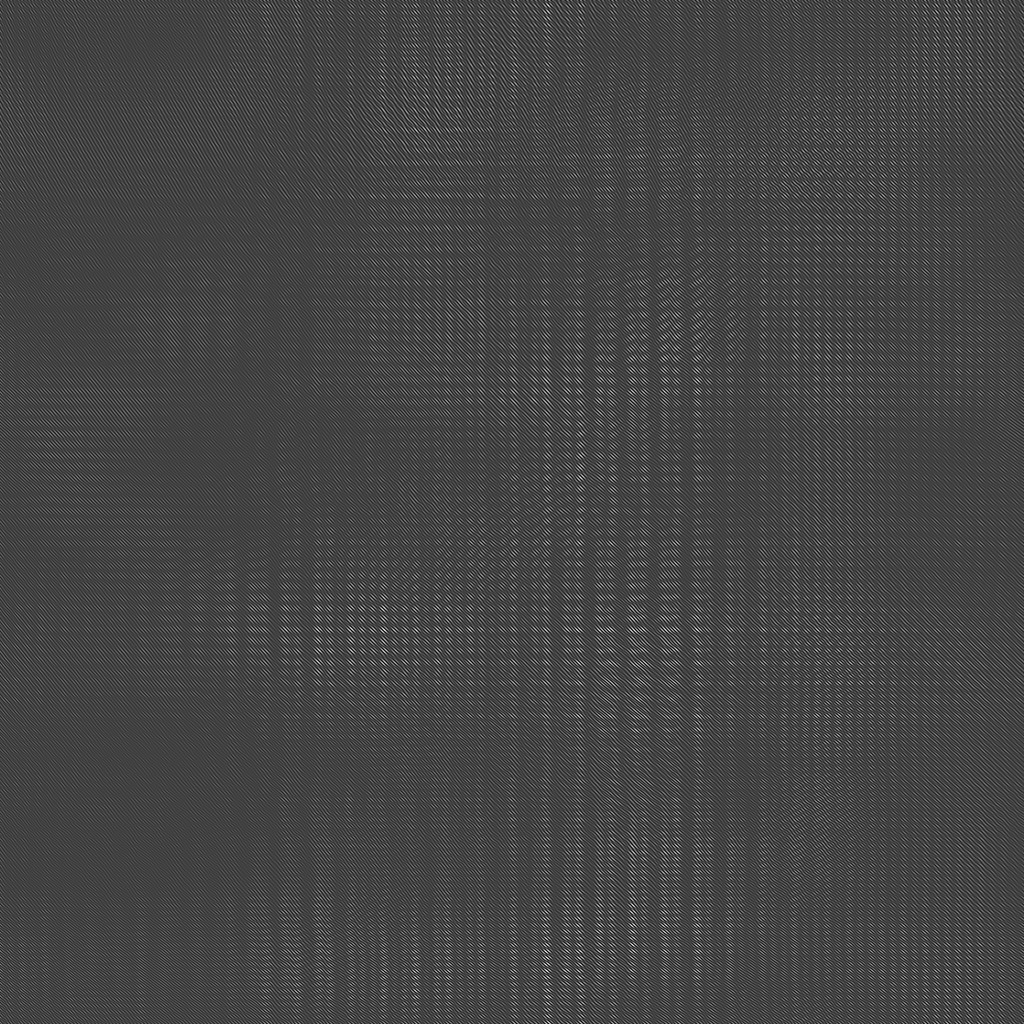
\includegraphics[width=\linewidth]{数字全息实验数据/计算机模拟全息/用软件模拟得到的全息图/2-大恒光电-全息图.jpg}
    \subcaption{计算机模拟的全息图}
  \end{subfigure}
  \begin{subfigure}{.32\textwidth}
    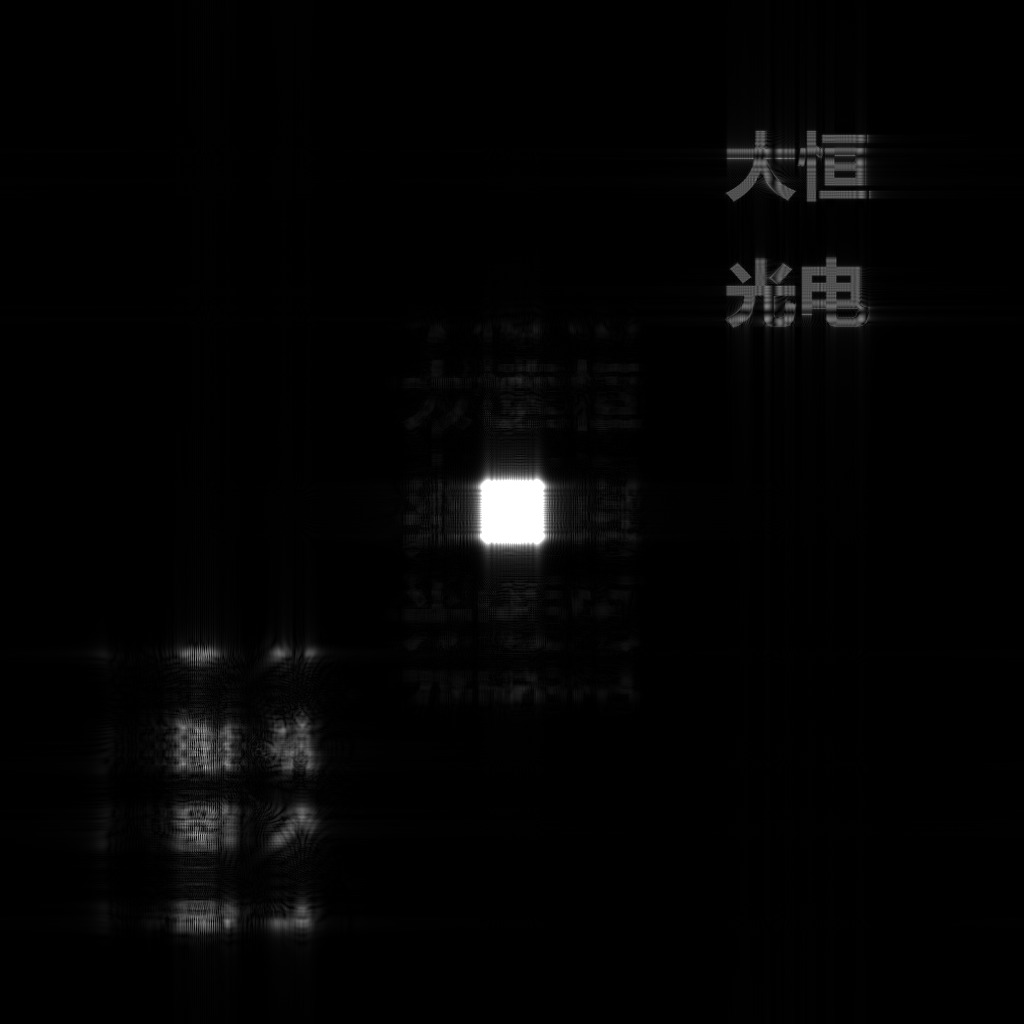
\includegraphics[width=\linewidth]{数字全息实验数据/计算机模拟全息/用软件重建的结果图像/2-大恒光电-重建.jpg}
    \subcaption{计算机重建结果}
  \end{subfigure}
  \caption{计算机模拟全息实验图像-大恒光电}
\end{figure}

\begin{figure}[H]
  \centering
  \begin{subfigure}{.32\textwidth}
    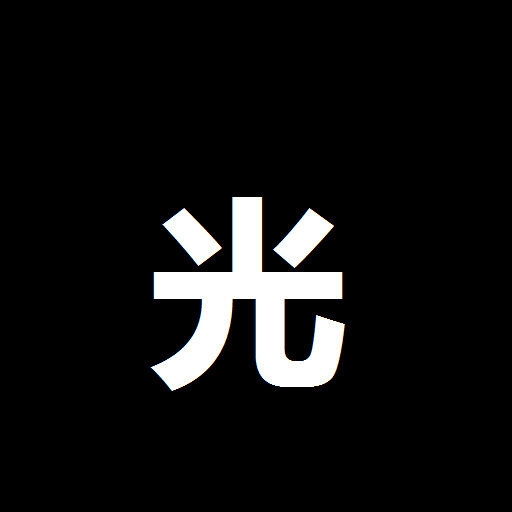
\includegraphics[width=\linewidth]{数字全息实验数据/计算机模拟全息/全息样品图片/3-光.jpg}
    \subcaption{使用的原图}
  \end{subfigure}
  \begin{subfigure}{.32\textwidth}
    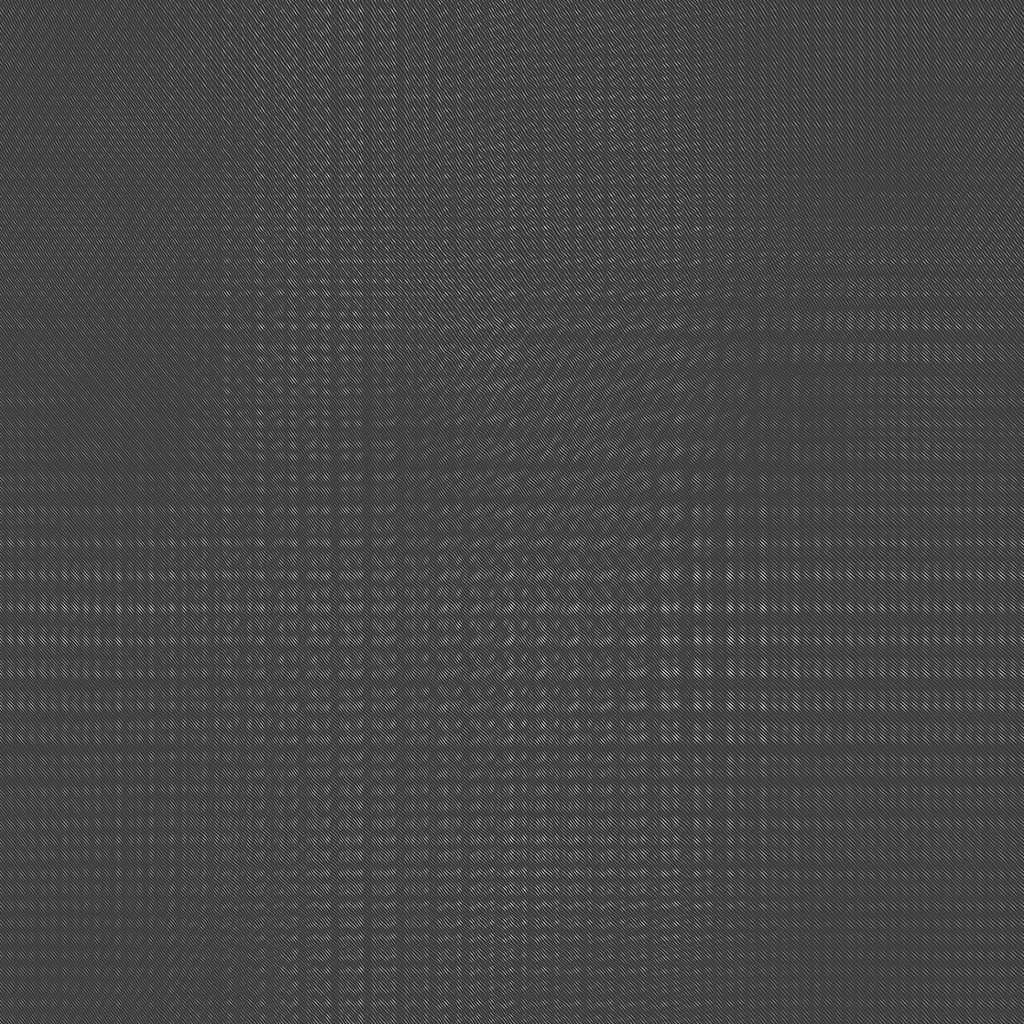
\includegraphics[width=\linewidth]{数字全息实验数据/计算机模拟全息/用软件模拟得到的全息图/3-光-全息图.jpg}
    \subcaption{计算机模拟的全息图}
  \end{subfigure}
  \begin{subfigure}{.32\textwidth}
    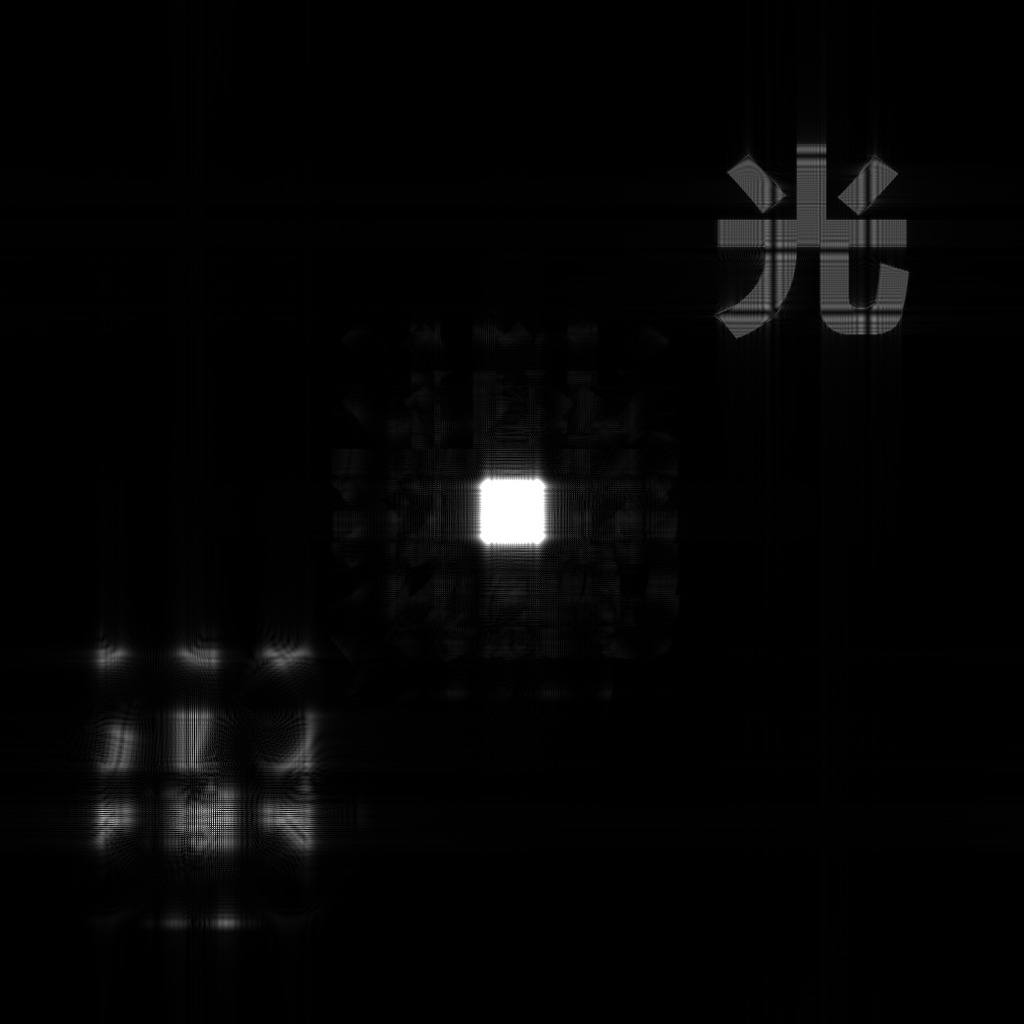
\includegraphics[width=\linewidth]{数字全息实验数据/计算机模拟全息/用软件重建的结果图像/3-光-重建.jpg}
    \subcaption{计算机重建结果}
  \end{subfigure}
  \caption{计算机模拟全息实验图像-光}
\end{figure}

\begin{figure}[H]
  \centering
  \begin{subfigure}{.32\textwidth}
    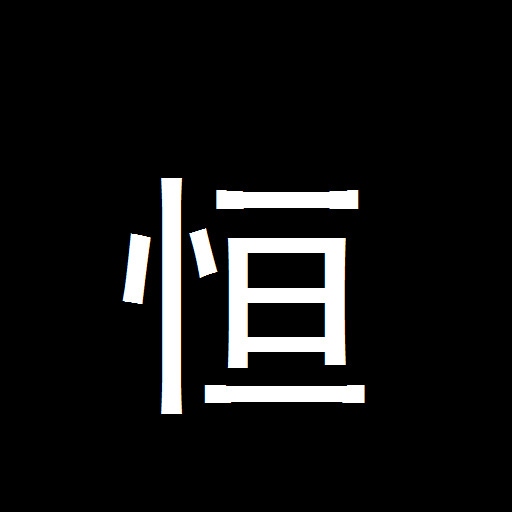
\includegraphics[width=\linewidth]{数字全息实验数据/计算机模拟全息/全息样品图片/4-恒.jpg}
    \subcaption{使用的原图}
  \end{subfigure}
  \begin{subfigure}{.32\textwidth}
    
\includegraphics[width=\linewidth]{数字全息实验数据/计算机模拟全息/用软件模拟得到的全息图/4-恒-全息图.jpg}
    \subcaption{计算机模拟的全息图}
  \end{subfigure}
  \begin{subfigure}{.32\textwidth}
    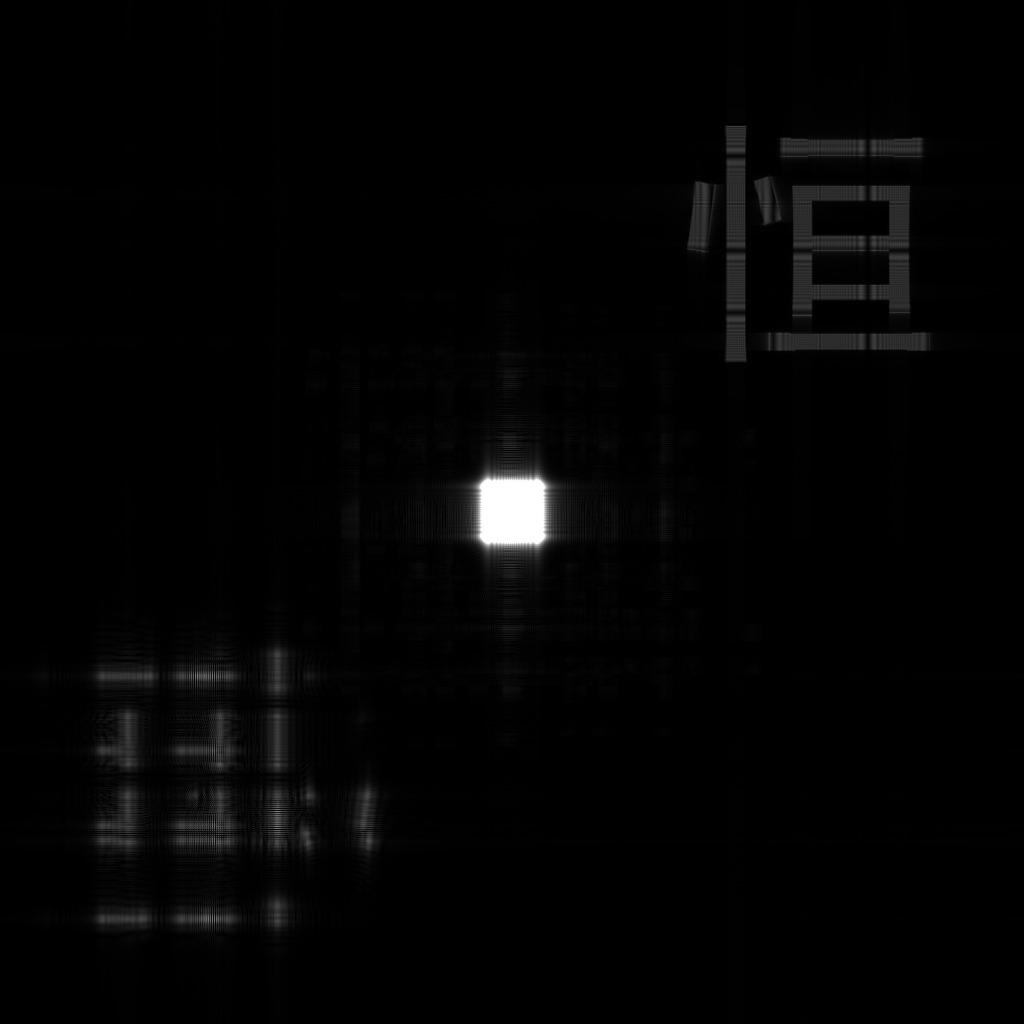
\includegraphics[width=\linewidth]{数字全息实验数据/计算机模拟全息/用软件重建的结果图像/4-恒-重建.jpg}
    \subcaption{计算机重建结果}
  \end{subfigure}
  \caption{计算机模拟全息实验图像-恒}
\end{figure}

\begin{figure}[H]
  \centering
  \begin{subfigure}{.32\textwidth}
    
\includegraphics[width=\linewidth]{数字全息实验数据/计算机模拟全息/全息样品图片/5-敏.jpg}
    \subcaption{使用的原图}
  \end{subfigure}
  \begin{subfigure}{.32\textwidth}
    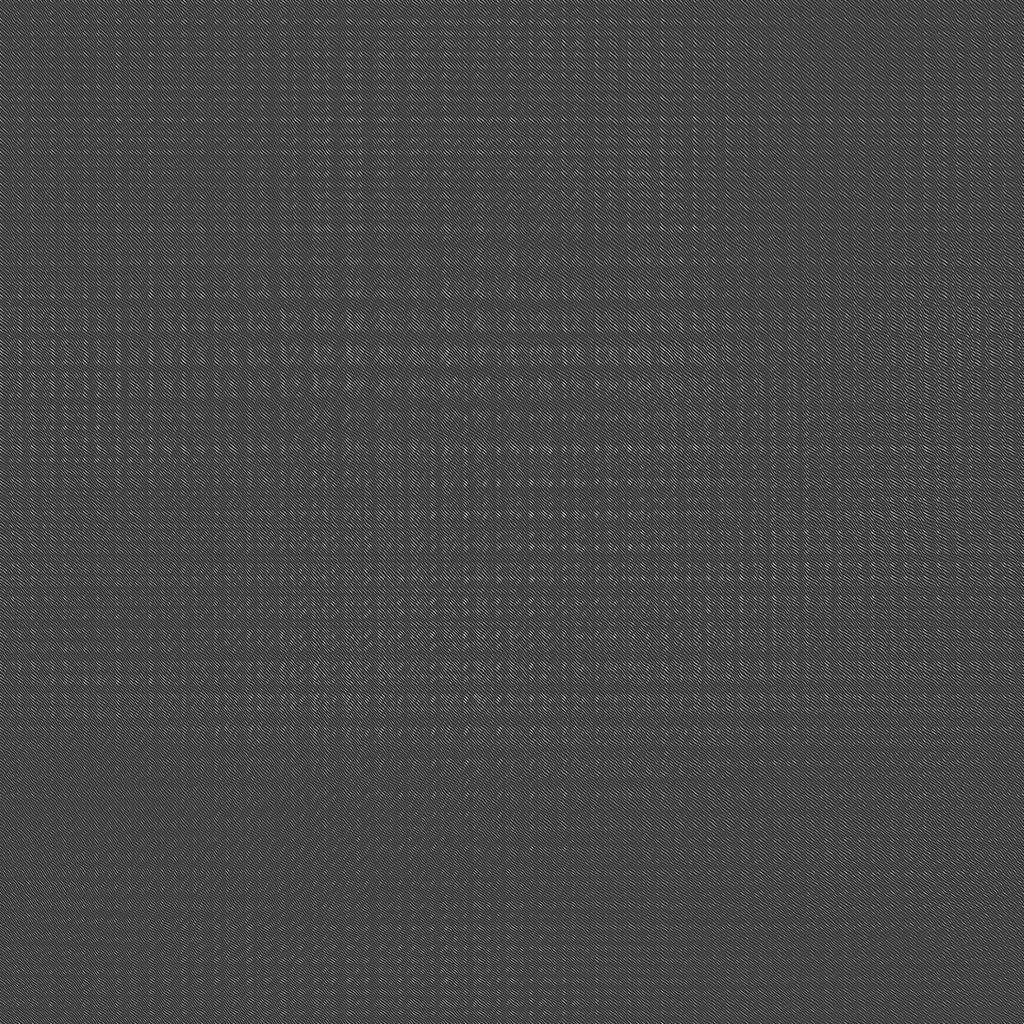
\includegraphics[width=\linewidth]{数字全息实验数据/计算机模拟全息/用软件模拟得到的全息图/5-敏-全息图.jpg}
    \subcaption{计算机模拟的全息图}
  \end{subfigure}
  \begin{subfigure}{.32\textwidth}
    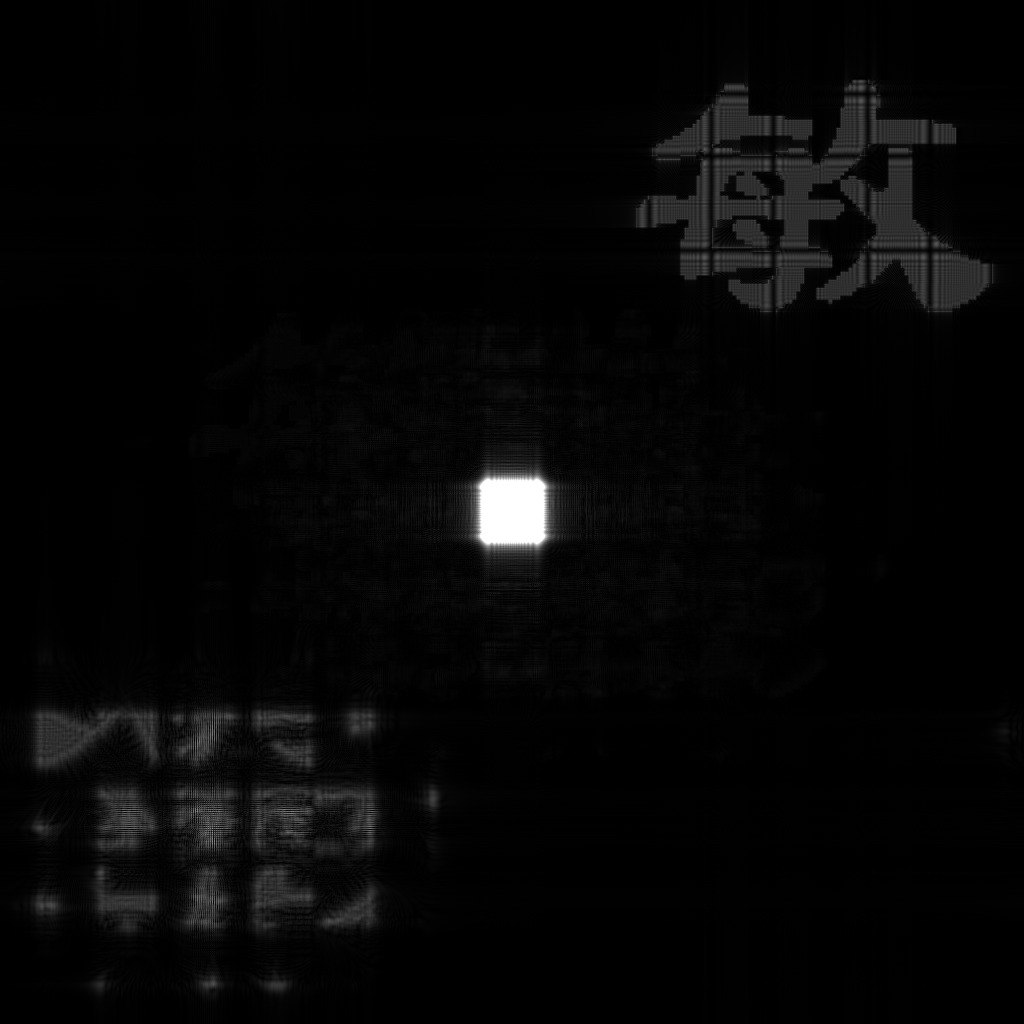
\includegraphics[width=\linewidth]{数字全息实验数据/计算机模拟全息/用软件重建的结果图像/5-敏-重建.jpg}
    \subcaption{计算机重建结果}
  \end{subfigure}
  \caption{计算机模拟全息实验图像-敏}
\end{figure}

再现得到的结果图像是理想的结果,有一个清晰的像,一个模糊的像。清晰的那个应该是正一级虚像,模糊的那个应该是负一级实像。

\subsection{可视数字全息}

用上一个实验得到的计算机模拟出来的全息图像,搭建全息再现光路,把全息图放在光路里,之后用摄像机观察光路重构出的图像。

实验中使用的全息图和光路再现出的原图如下

\begin{figure}[H]
  \centering
  \begin{subfigure}{.48\textwidth}
    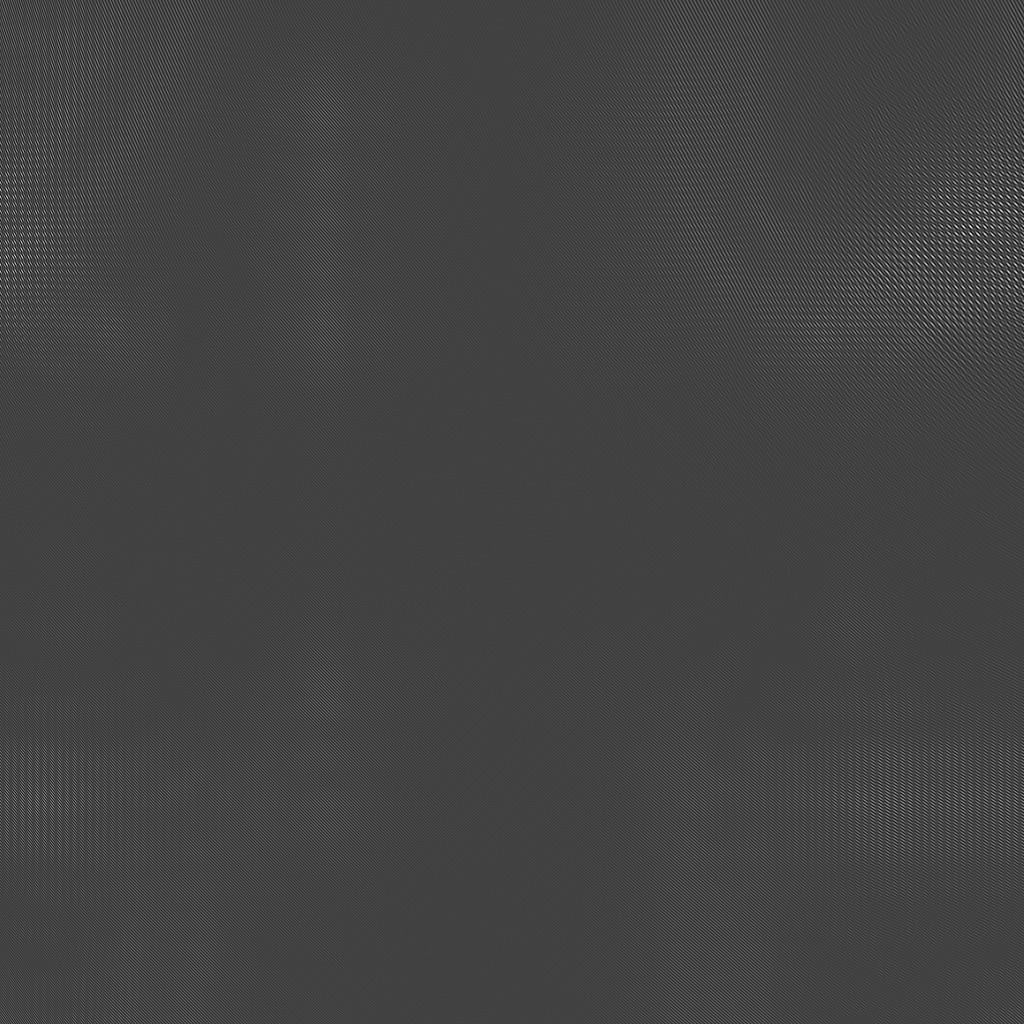
\includegraphics[width=\linewidth]{数字全息实验数据/可视数字全息/实验中使用的全息图-大恒.jpg}
    \subcaption{实验中使用的全息图}
  \end{subfigure}
  \begin{subfigure}{.48\textwidth}
    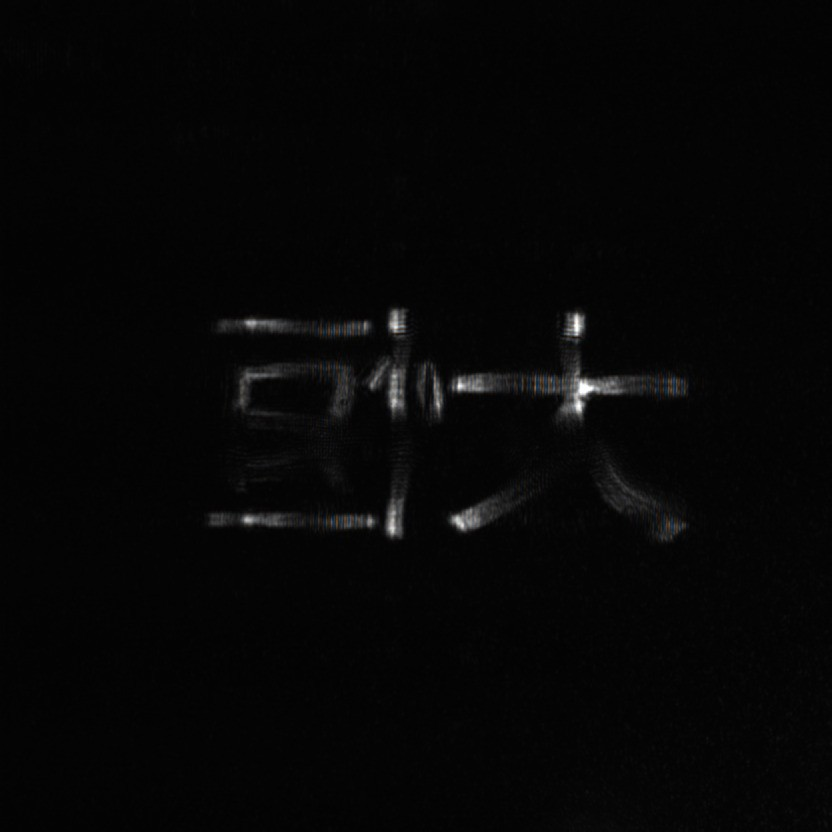
\includegraphics[width=\linewidth]{数字全息实验数据/可视数字全息/原图-大恒.jpg}
    \subcaption{光路重建结果}
  \end{subfigure}
  \caption{可视数字全息实验图像-大恒}
\end{figure}

\begin{figure}[H]
  \centering
  \begin{subfigure}{.48\textwidth}
    
\includegraphics[width=\linewidth]{数字全息实验数据/可视数字全息/实验中使用的全息图-恒.jpg}
    \subcaption{实验中使用的全息图}
  \end{subfigure}
  \begin{subfigure}{.48\textwidth}
    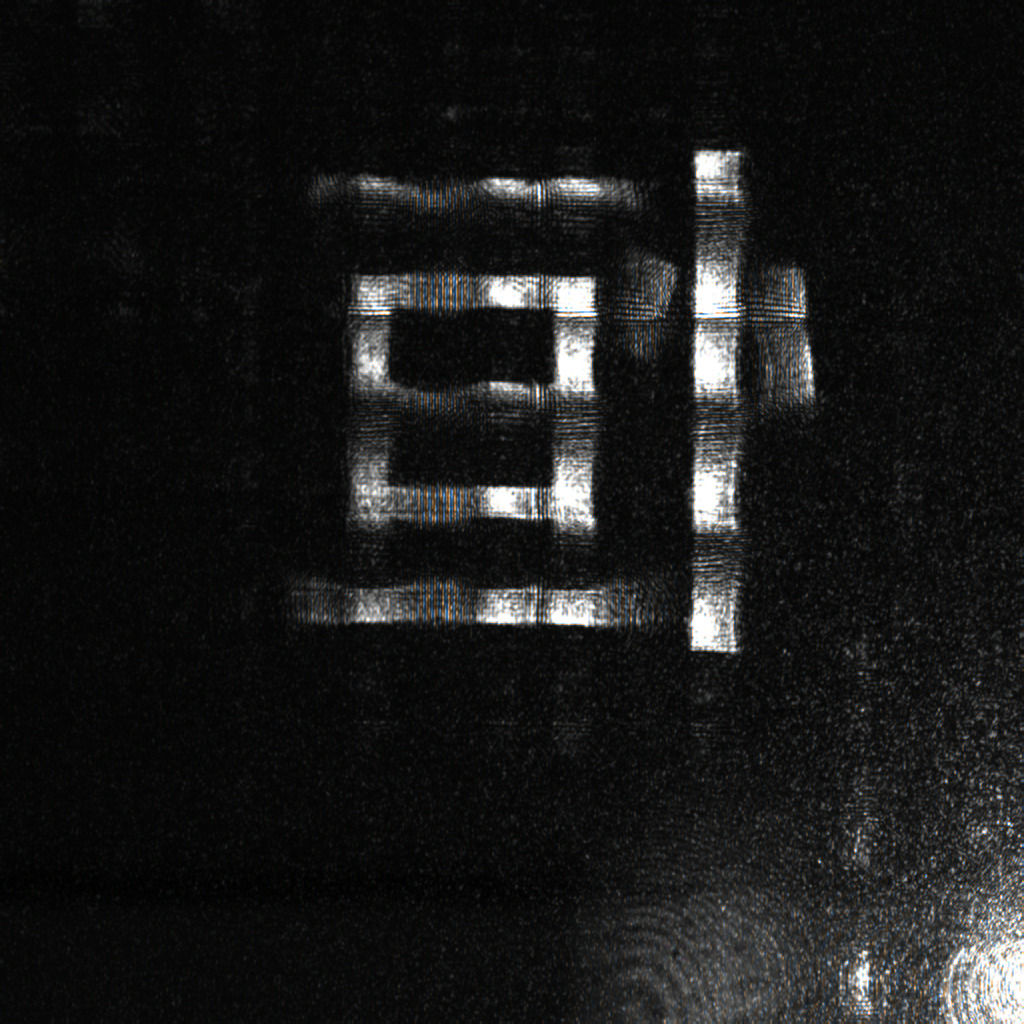
\includegraphics[width=\linewidth]{数字全息实验数据/可视数字全息/原图-恒.jpg}
    \subcaption{光路重建结果}
  \end{subfigure}
  \caption{可视数字全息实验图像-恒}
\end{figure}

\subsection{数字全息}

搭建全息干涉光路,之后生成全息图像,将生成的全息图像用摄像机拍摄下来,用计算机对全息图进行重构,得到原来的图像。

下面是我们的实验数据,左边的图是摄像机拍摄到的全息图,右面的是计算机根据全息图还原的图像。

\begin{figure}[H]
  \centering
  \begin{subfigure}{.48\textwidth}
    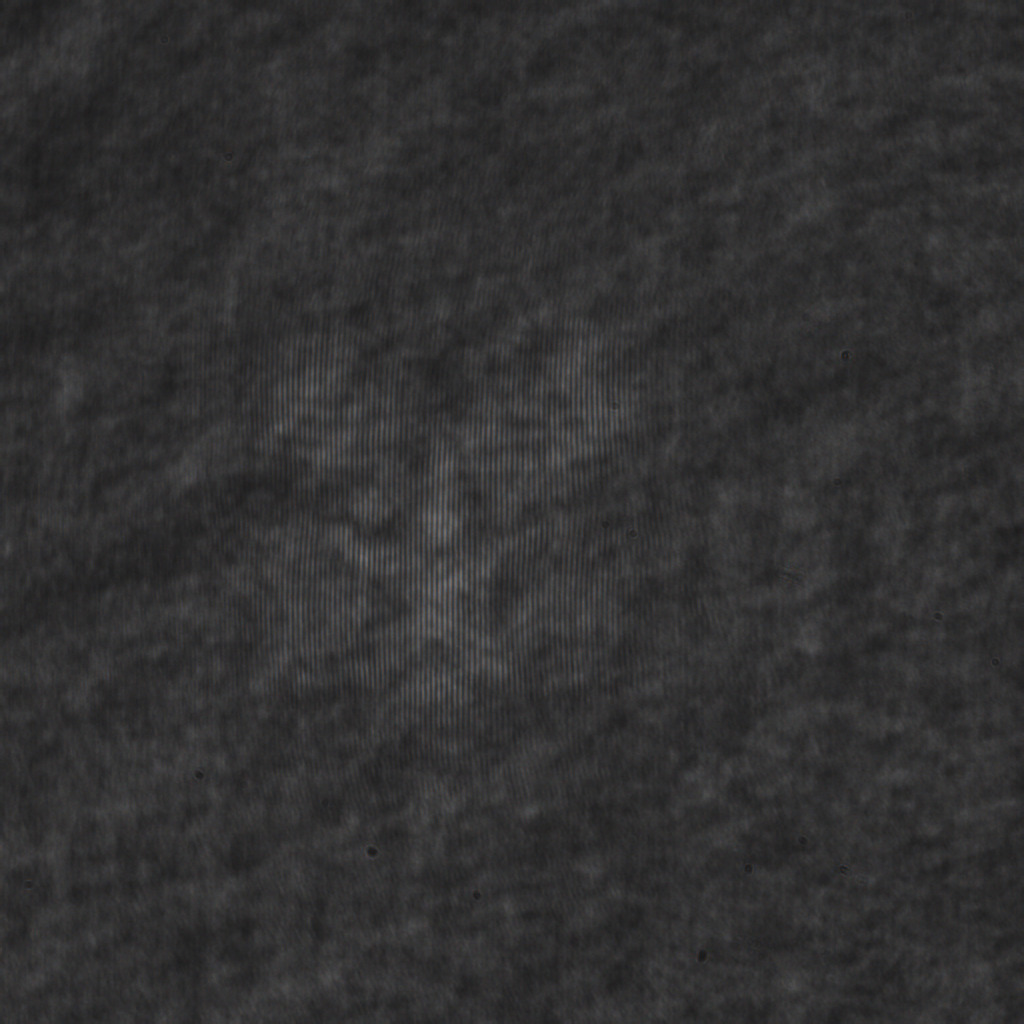
\includegraphics[width=\linewidth]{数字全息实验数据/数字全息/大1/大1.jpg}
    \subcaption{实验中拍摄的全息图}
  \end{subfigure}
  \begin{subfigure}{.48\textwidth}
    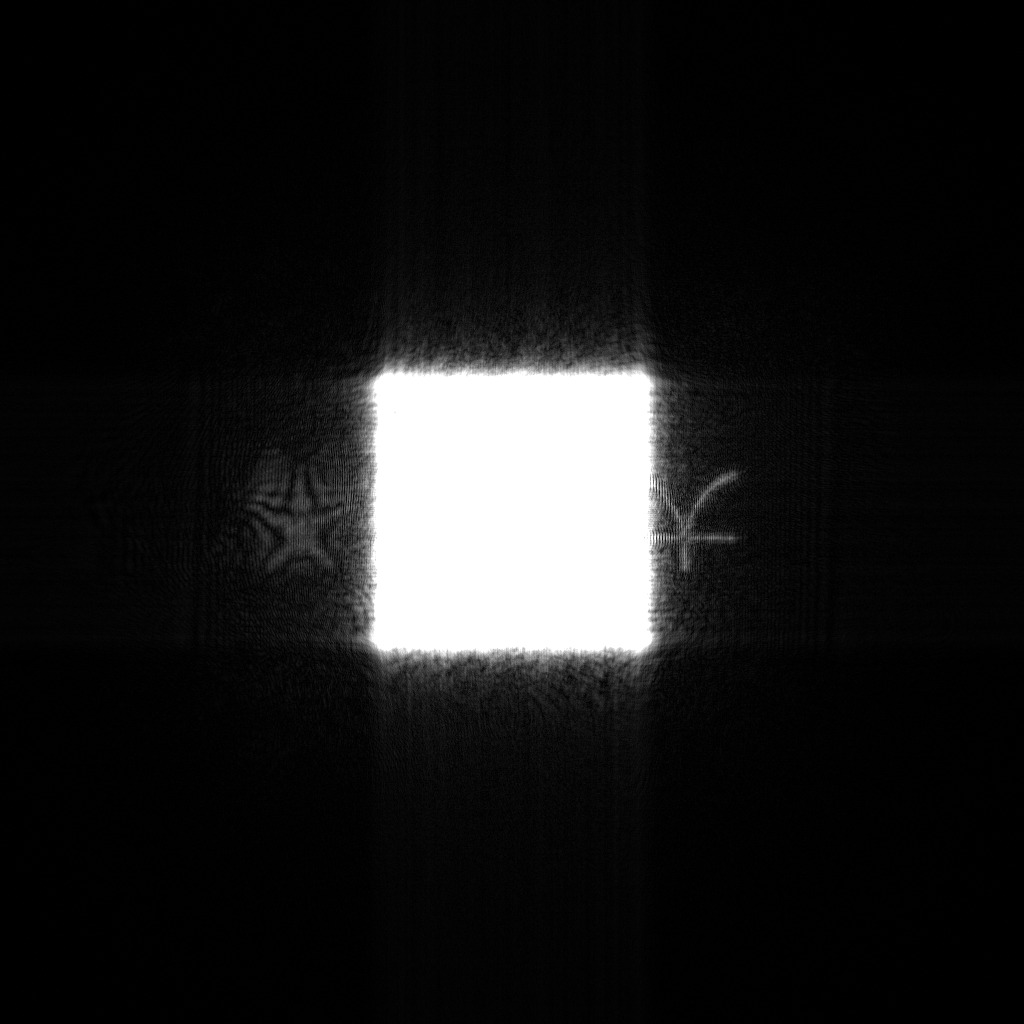
\includegraphics[width=\linewidth]{数字全息实验数据/数字全息/大1/数字全息输出结果-大1.jpg}
    \subcaption{计算机重建结果}
  \end{subfigure}
  \caption{数字全息实验图像-大(第一组实验)}
\end{figure}

\begin{figure}[H]
  \centering
  \begin{subfigure}{.48\textwidth}
    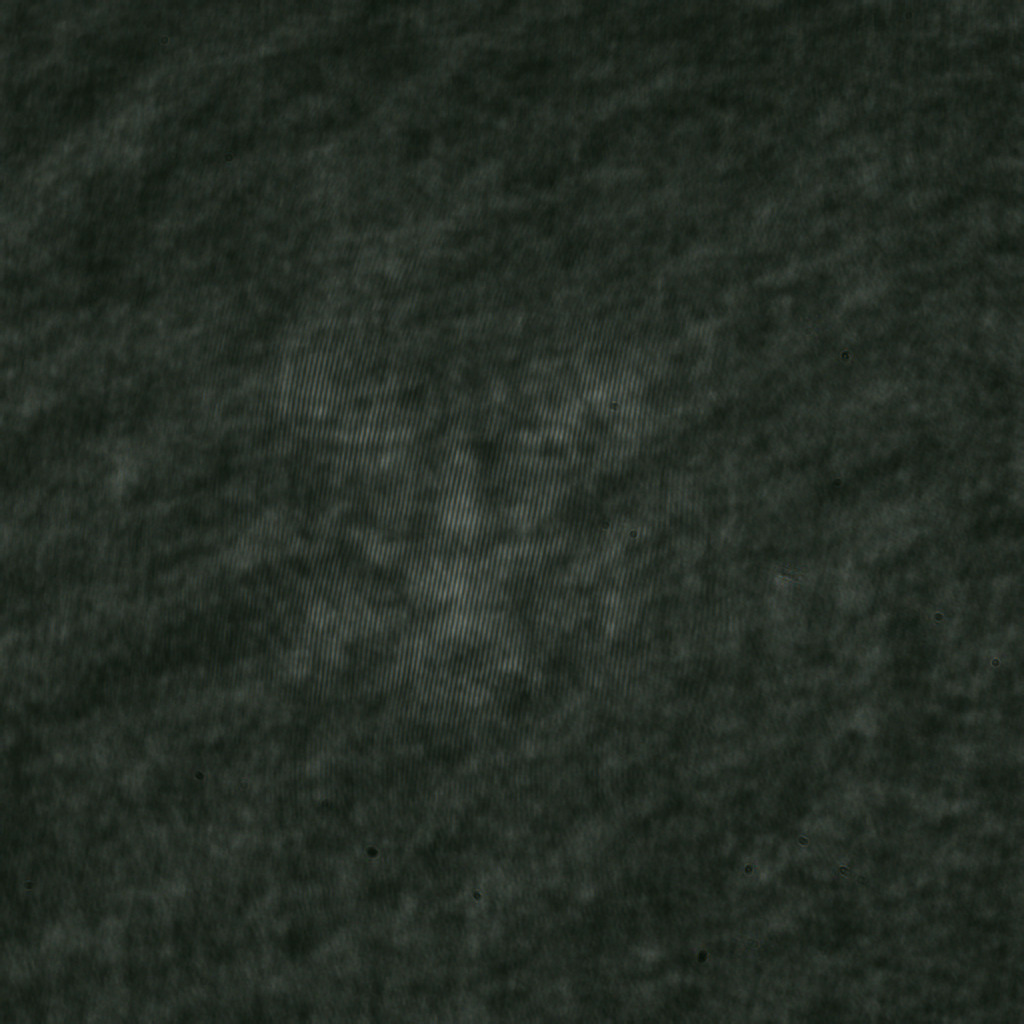
\includegraphics[width=\linewidth]{数字全息实验数据/数字全息/大2/大2.jpg}
    \subcaption{实验中拍摄的全息图}
  \end{subfigure}
  \begin{subfigure}{.48\textwidth}
    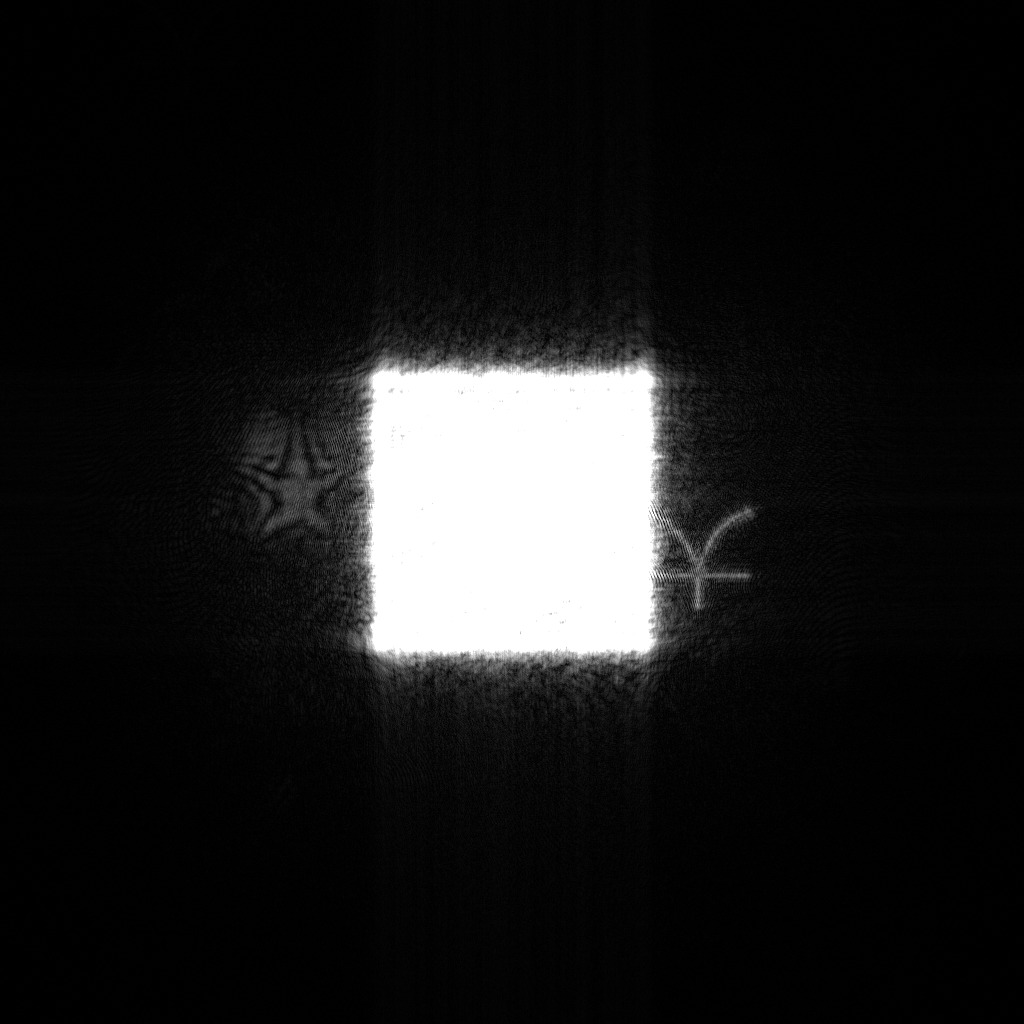
\includegraphics[width=\linewidth]{数字全息实验数据/数字全息/大2/数字全息输出结果-大2.jpg}
    \subcaption{计算机重建结果}
  \end{subfigure}
  \caption{数字全息实验图像-大(第二组实验)}
\end{figure}

\begin{figure}[H]
  \centering
  \begin{subfigure}{.48\textwidth}
    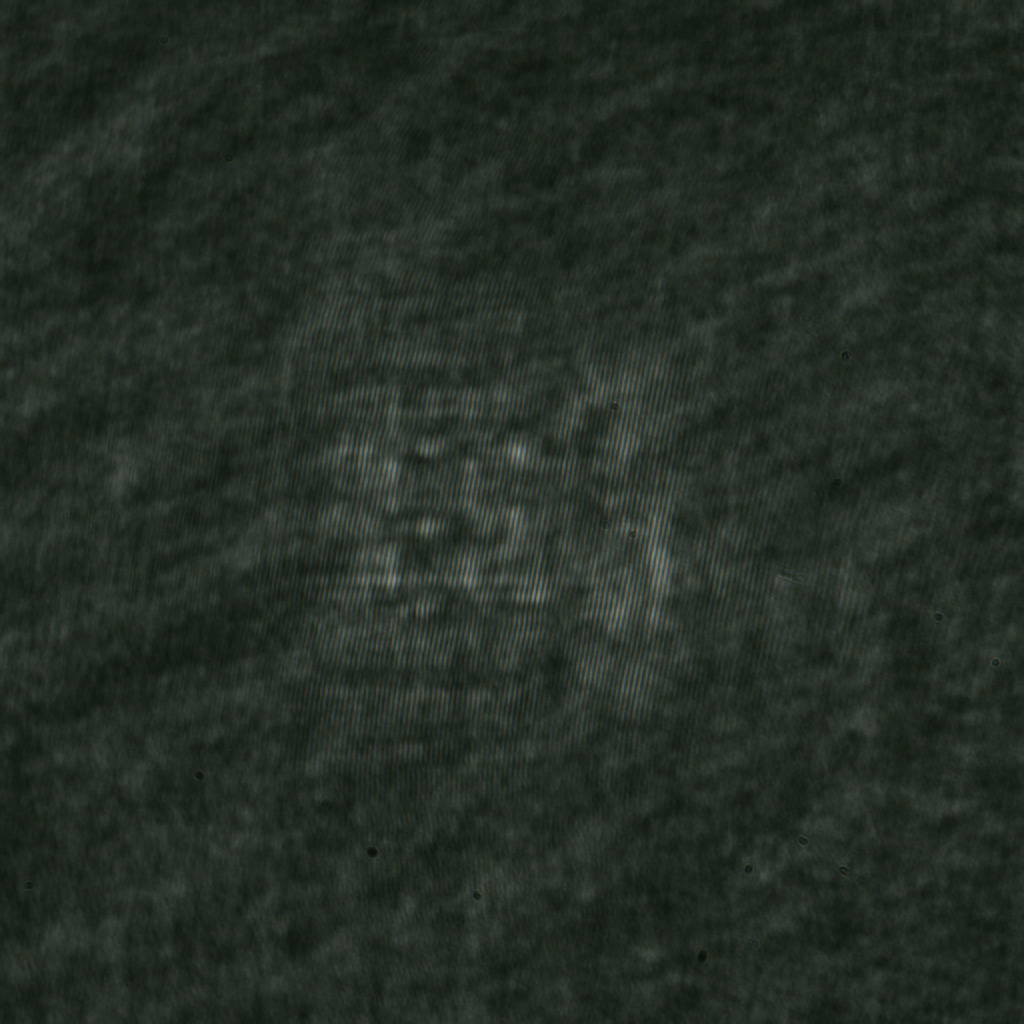
\includegraphics[width=\linewidth]{数字全息实验数据/数字全息/恒/恒.jpg}
    \subcaption{实验中拍摄的全息图}
  \end{subfigure}
  \begin{subfigure}{.48\textwidth}
    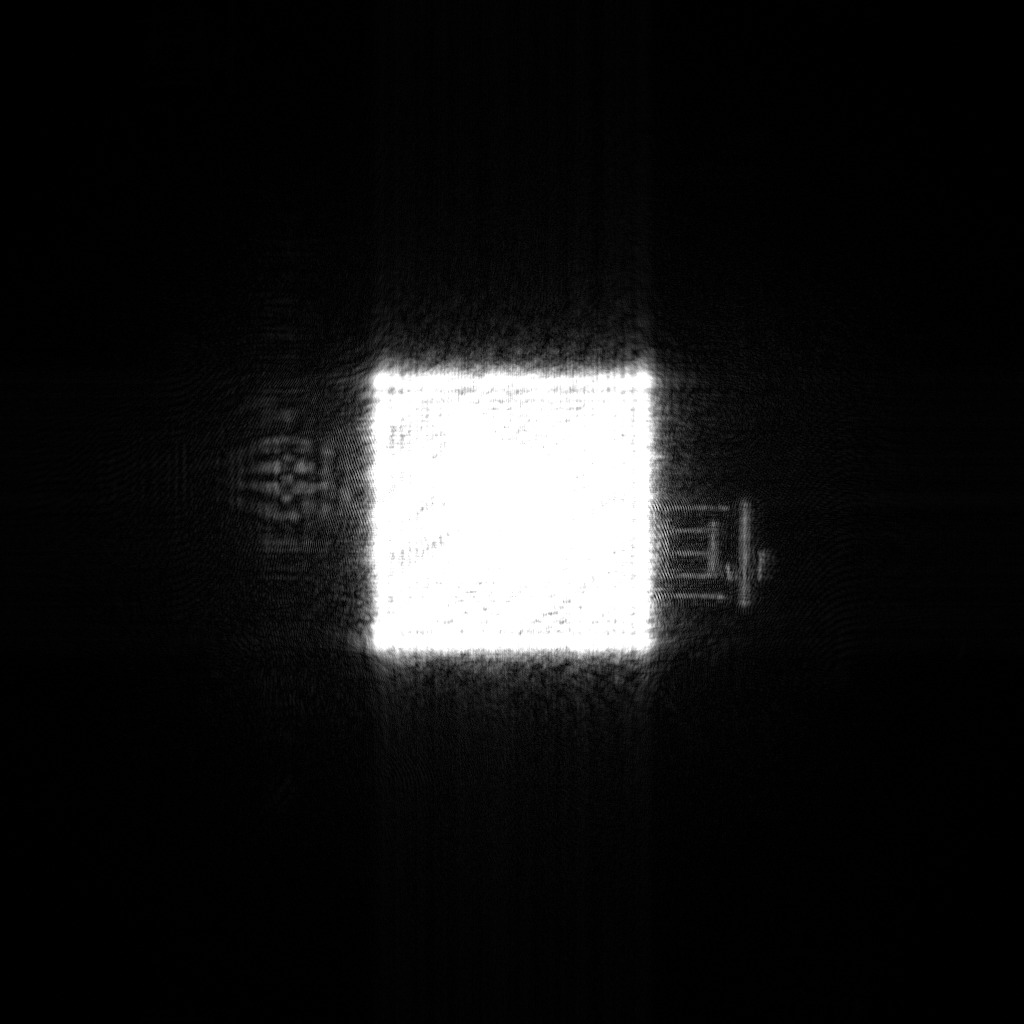
\includegraphics[width=\linewidth]{数字全息实验数据/数字全息/恒/数字全息输出结果-恒.jpg}
    \subcaption{计算机重建结果}
  \end{subfigure}
  \caption{数字全息实验图像-恒}
\end{figure}

实验中发现图像和中间的方框重合了,可能是选的角度不是很好。

\subsection{实时传统全息}

将上面的数字全息实验得到的用光路生成的全息图,加载到上面可视数字全息的光路中,用光路重建光路生成的全息图。下面是几组实验结果。


\section{实验中遇到的问题及解决方法}

实验中主演遇到的问题就是光路的调节问题,这个光路的调节要领就是每一步都要极度准确,每放下一个镜子,镜子反射回去的光必须能和上一个镜子重合。同时,调节准直的时候需要在尽可能远的地方观察,在极远处光斑大小和近处应该一样。

\begin{figure}[H]
  \centering
  \begin{subfigure}{.48\textwidth}
    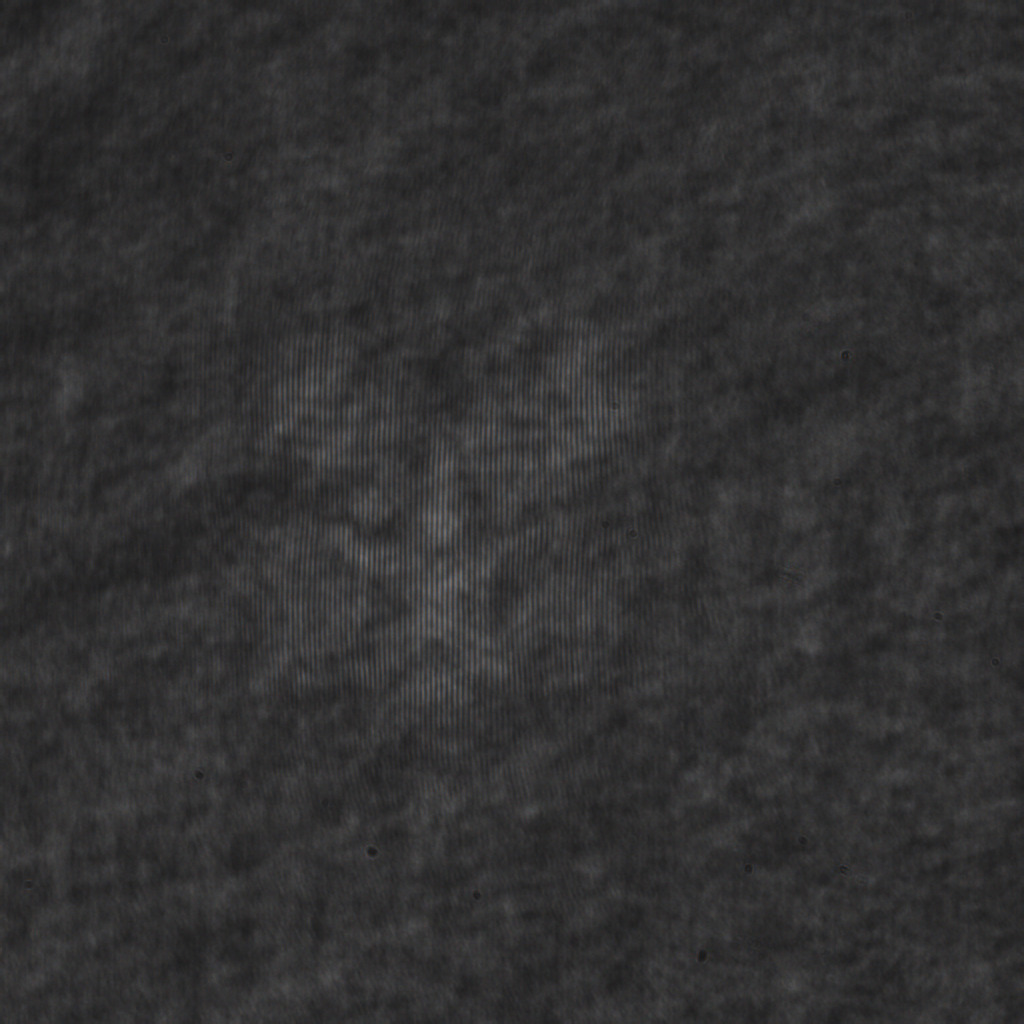
\includegraphics[width=\linewidth]{数字全息实验数据/数字全息/大1/大1.jpg}
    \subcaption{实验中使用的全息图}
  \end{subfigure}
  \begin{subfigure}{.48\textwidth}
    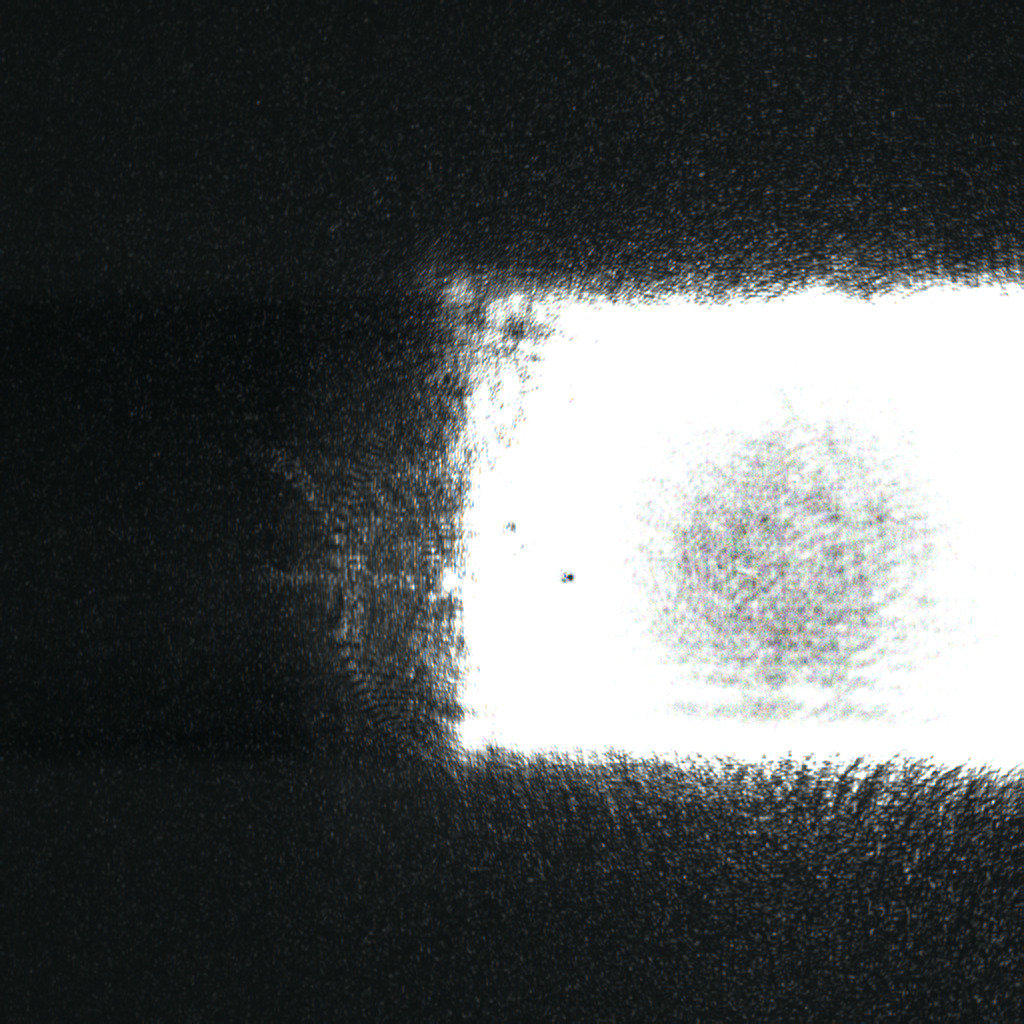
\includegraphics[width=\linewidth]{数字全息实验数据/实时传统全息/大1结果.jpg}
    \subcaption{光路重建结果}
  \end{subfigure}
  \caption{实时传统全息实验图像-大(第一组实验)}
\end{figure}

\begin{figure}[H]
  \centering
  \begin{subfigure}{.48\textwidth}
    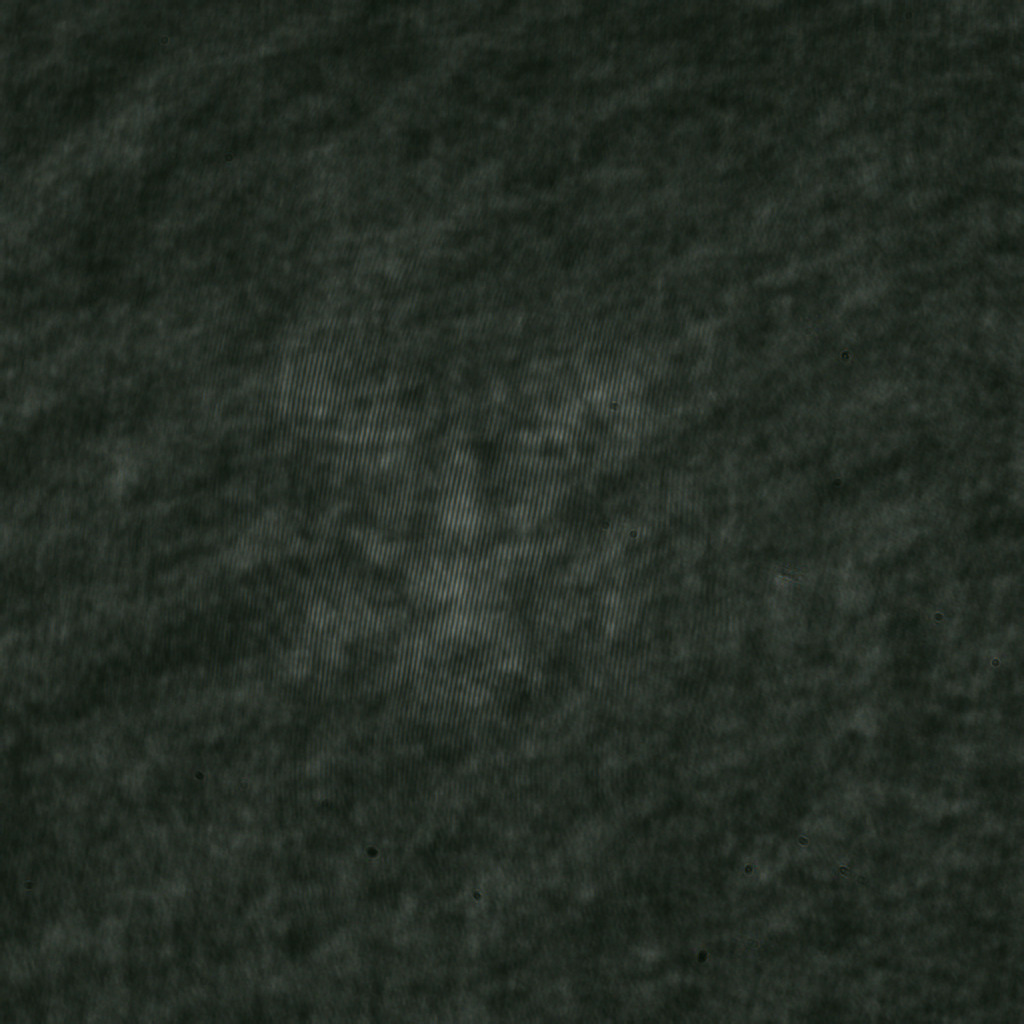
\includegraphics[width=\linewidth]{数字全息实验数据/数字全息/大2/大2.jpg}
    \subcaption{实验中使用的全息图}
  \end{subfigure}
  \begin{subfigure}{.48\textwidth}
    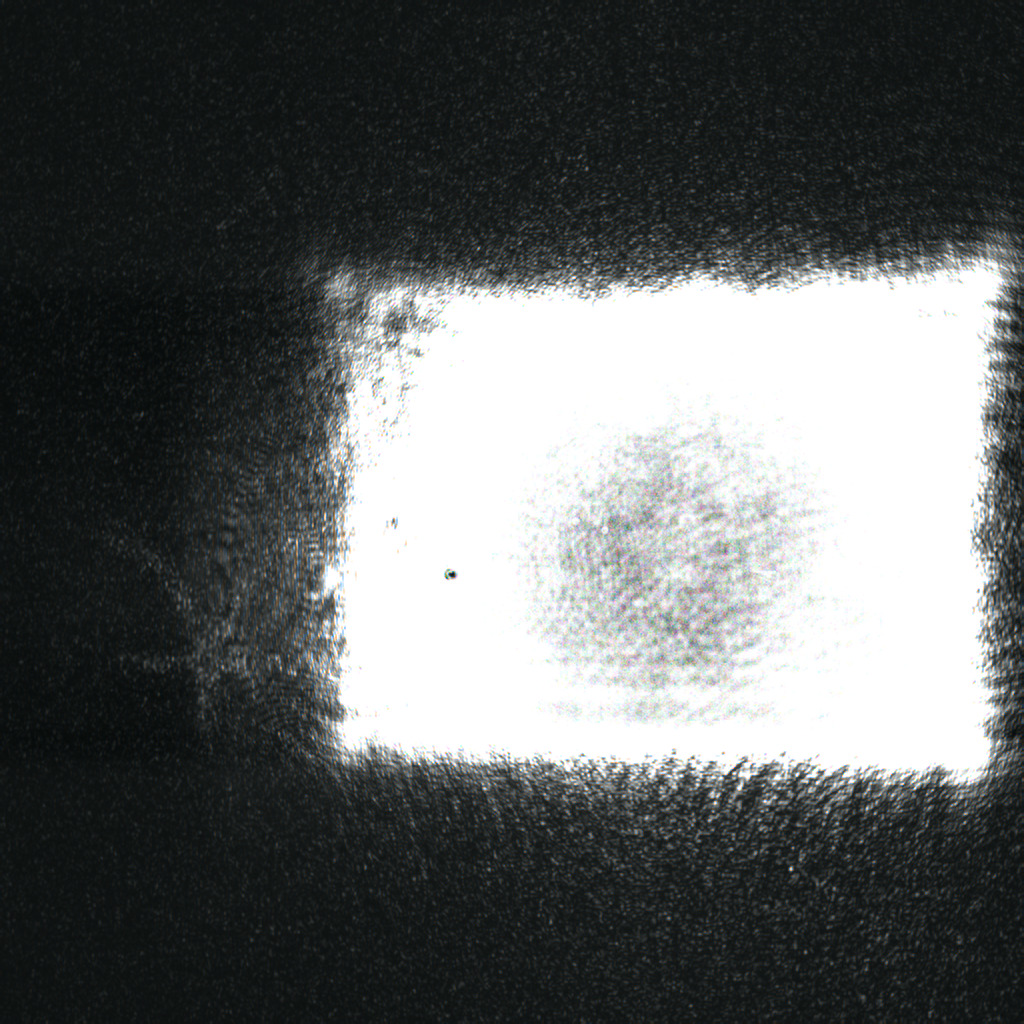
\includegraphics[width=\linewidth]{数字全息实验数据/实时传统全息/大2结果.jpg}
    \subcaption{光路重建结果}
  \end{subfigure}
  \caption{实时传统全息实验图像-大(第二组实验)}
\end{figure}

\begin{figure}[H]
  \centering
  \begin{subfigure}{.48\textwidth}
    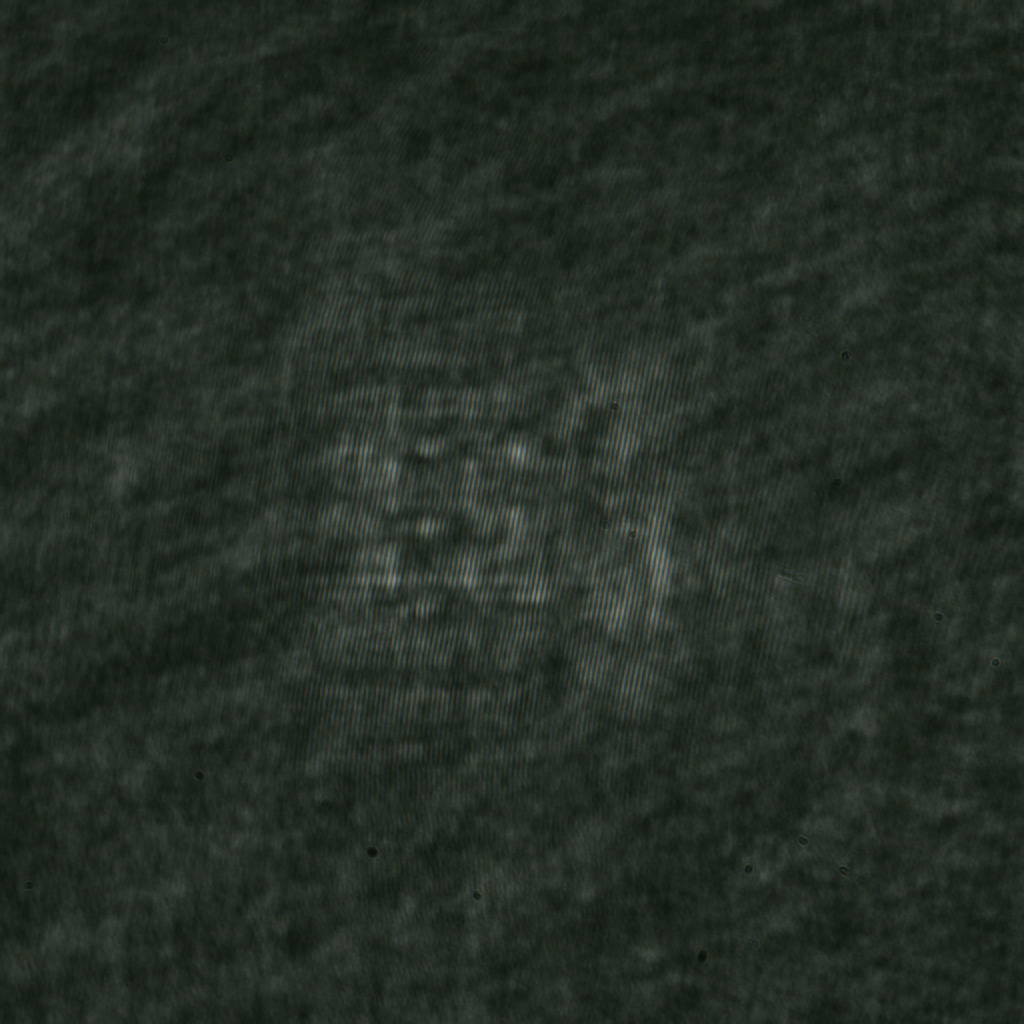
\includegraphics[width=\linewidth]{数字全息实验数据/数字全息/恒/恒.jpg}
    \subcaption{实验中使用的全息图}
  \end{subfigure}
  \begin{subfigure}{.48\textwidth}
    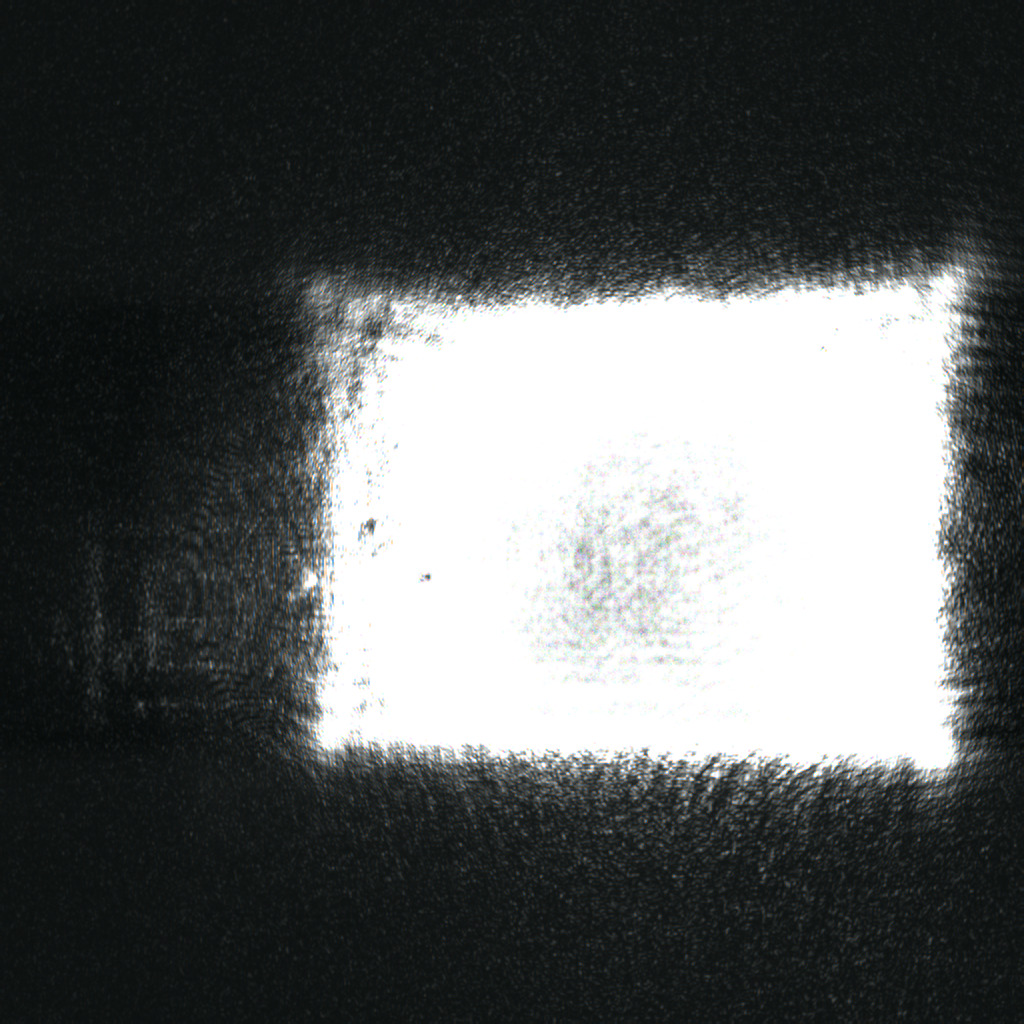
\includegraphics[width=\linewidth]{数字全息实验数据/实时传统全息/恒结果.jpg}
    \subcaption{光路重建结果}
  \end{subfigure}
  \caption{实时传统全息实验图像-恒}
\end{figure}

图像已经严重模糊但是尚且能辨认。

\section{参考文献}
\begin{itemize}[leftmargin=0pt]
  \item[] 近代物理实验讲义
\end{itemize}
\end{document} 

%%% Local Variables:
%%% mode: latex
%%% TeX-master: t
%%% End:
